\documentclass{article}
\usepackage{graphicx}

\title{Land Use, Structural Change and Urban Expansion: Fan-Out Fidelity Slice}
\author{F. Oswald}

\begin{document}
\maketitle

\section{Introduction}

This slice extracts two real Stata scripts from the published replication
package, both reading the same real input,
\texttt{data/raw/FRA\_base.dta} (French land-use/employment shares,
1806--2018): \texttt{code/stata/figure1.do} (Figure~\ref{fig:1} and two
appendix figures) and \texttt{code/stata/generatethetas.do}
(Figure~\ref{fig:7}, Figure~\ref{fig:a3} and Figure~\ref{fig:a4}).

\section{Results}

\begin{figure}[h]
\centering
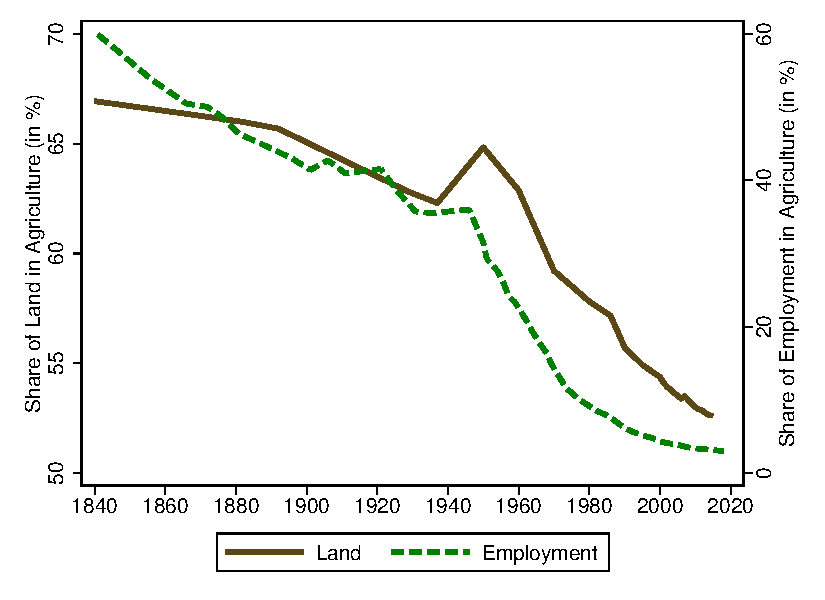
\includegraphics[width=0.7\textwidth]{output/data/plots/figure1.pdf}
\caption{Share of land and employment in agriculture}
\label{fig:1}
\end{figure}

\begin{figure}[h]
\centering
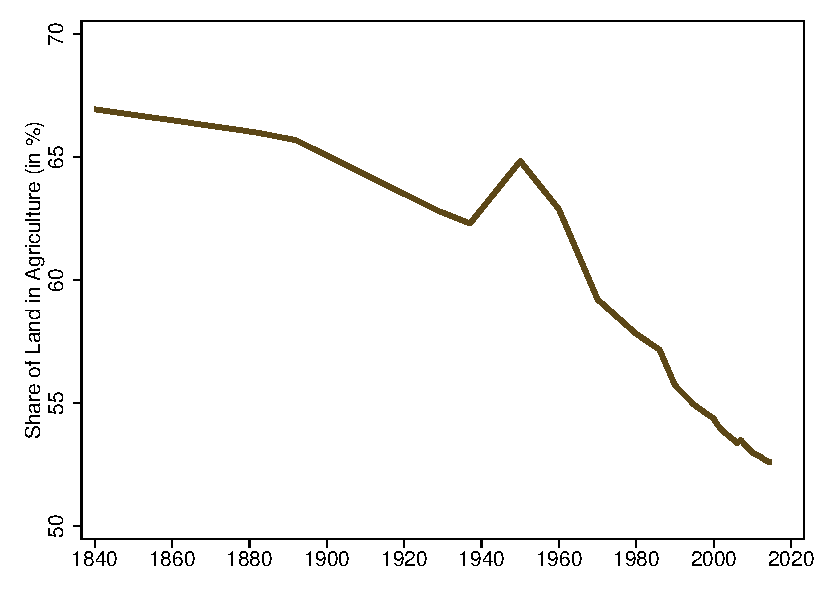
\includegraphics[width=0.7\textwidth]{output/data/plots/figureA2a.pdf}
\caption{Share of land in agriculture (Appendix A.2a)}
\label{fig:a2a}
\end{figure}

\begin{figure}[h]
\centering
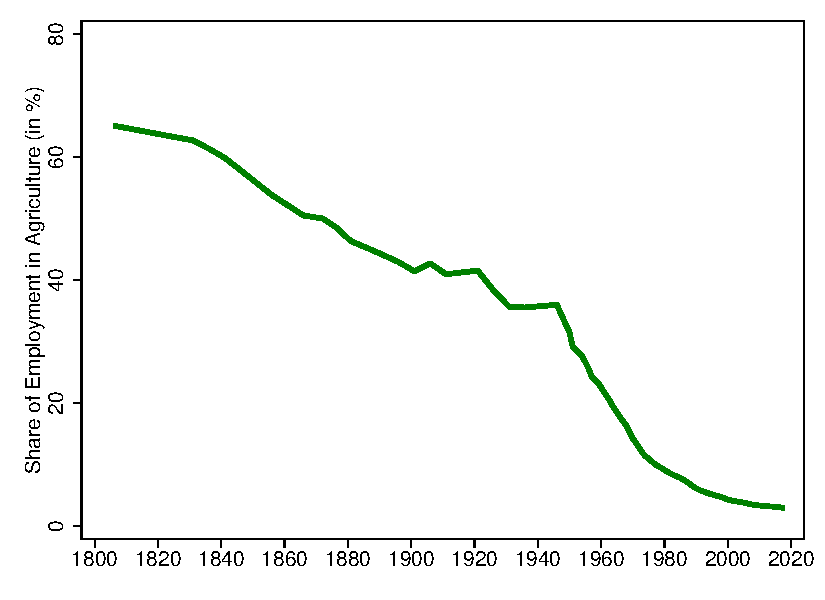
\includegraphics[width=0.7\textwidth]{output/data/plots/figureA2b.pdf}
\caption{Share of employment in agriculture (Appendix A.2b)}
\label{fig:a2b}
\end{figure}

\begin{figure}[h]
\centering
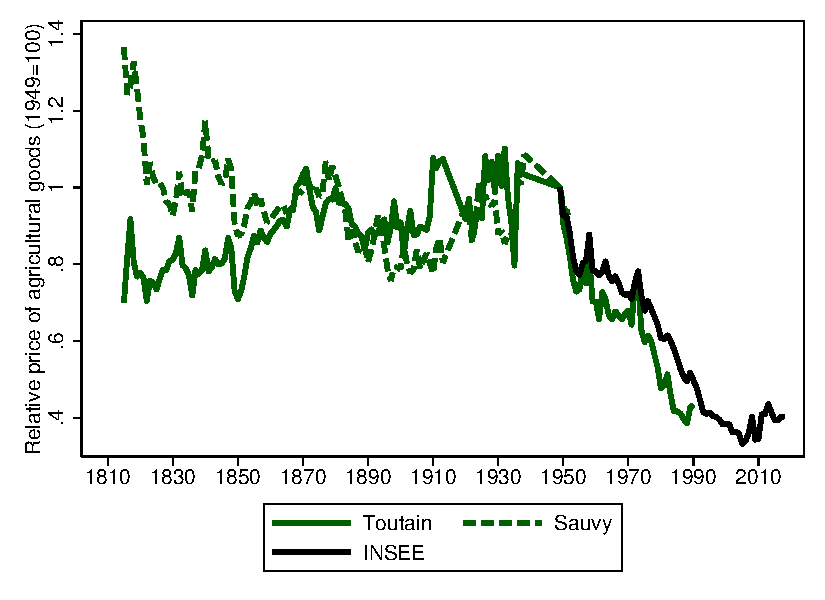
\includegraphics[width=0.7\textwidth]{output/data/plots/figureA3.pdf}
\caption{Relative price of agricultural goods (Appendix A.3)}
\label{fig:a3}
\end{figure}

\begin{figure}[h]
\centering
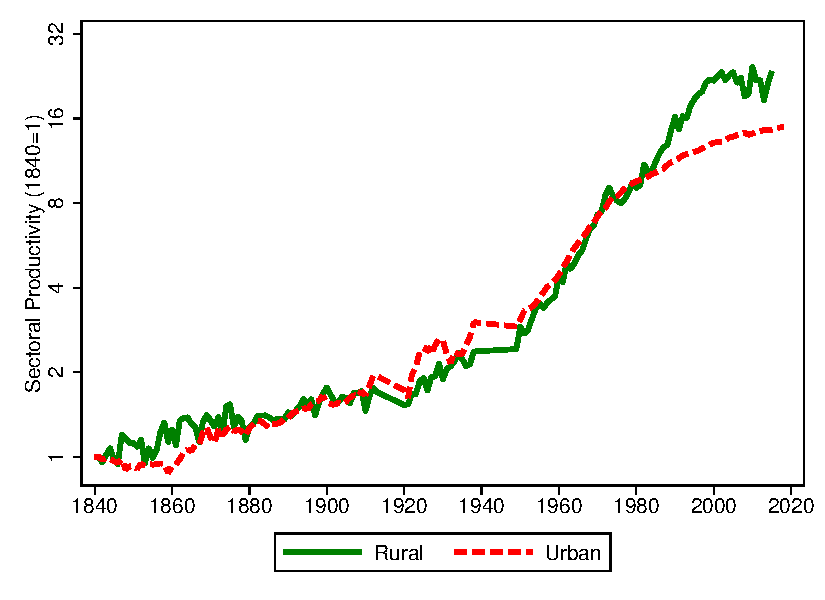
\includegraphics[width=0.7\textwidth]{output/data/plots/figure7.pdf}
\caption{Sectoral productivity, rural vs.\ urban}
\label{fig:7}
\end{figure}

\begin{figure}[h]
\centering
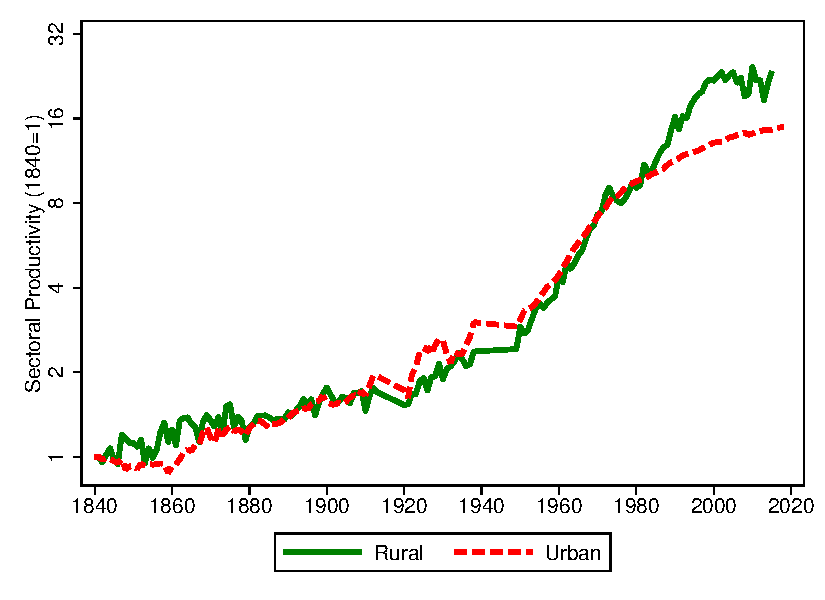
\includegraphics[width=0.7\textwidth]{output/data/plots/figureA4.pdf}
\caption{Sectoral productivity, rural vs.\ urban (Appendix A.4)}
\label{fig:a4}
\end{figure}

\end{document}
